\documentclass[11pt]{scrartcl}

\usepackage[sexy]{evan}
\usepackage{float}
\usepackage{graphicx}
\usepackage{amsmath}

\author{Axel Benjamin Rocca Cruz 20234046A}
\title{Tarea previa Cin\'etica Qu\'imica}

\begin{document}
\maketitle
\section{Realize un diagrama de bloques del experimento 1.}

\begin{figure}[H]
\begin{center}
	\caption{diagrama de flujo}
	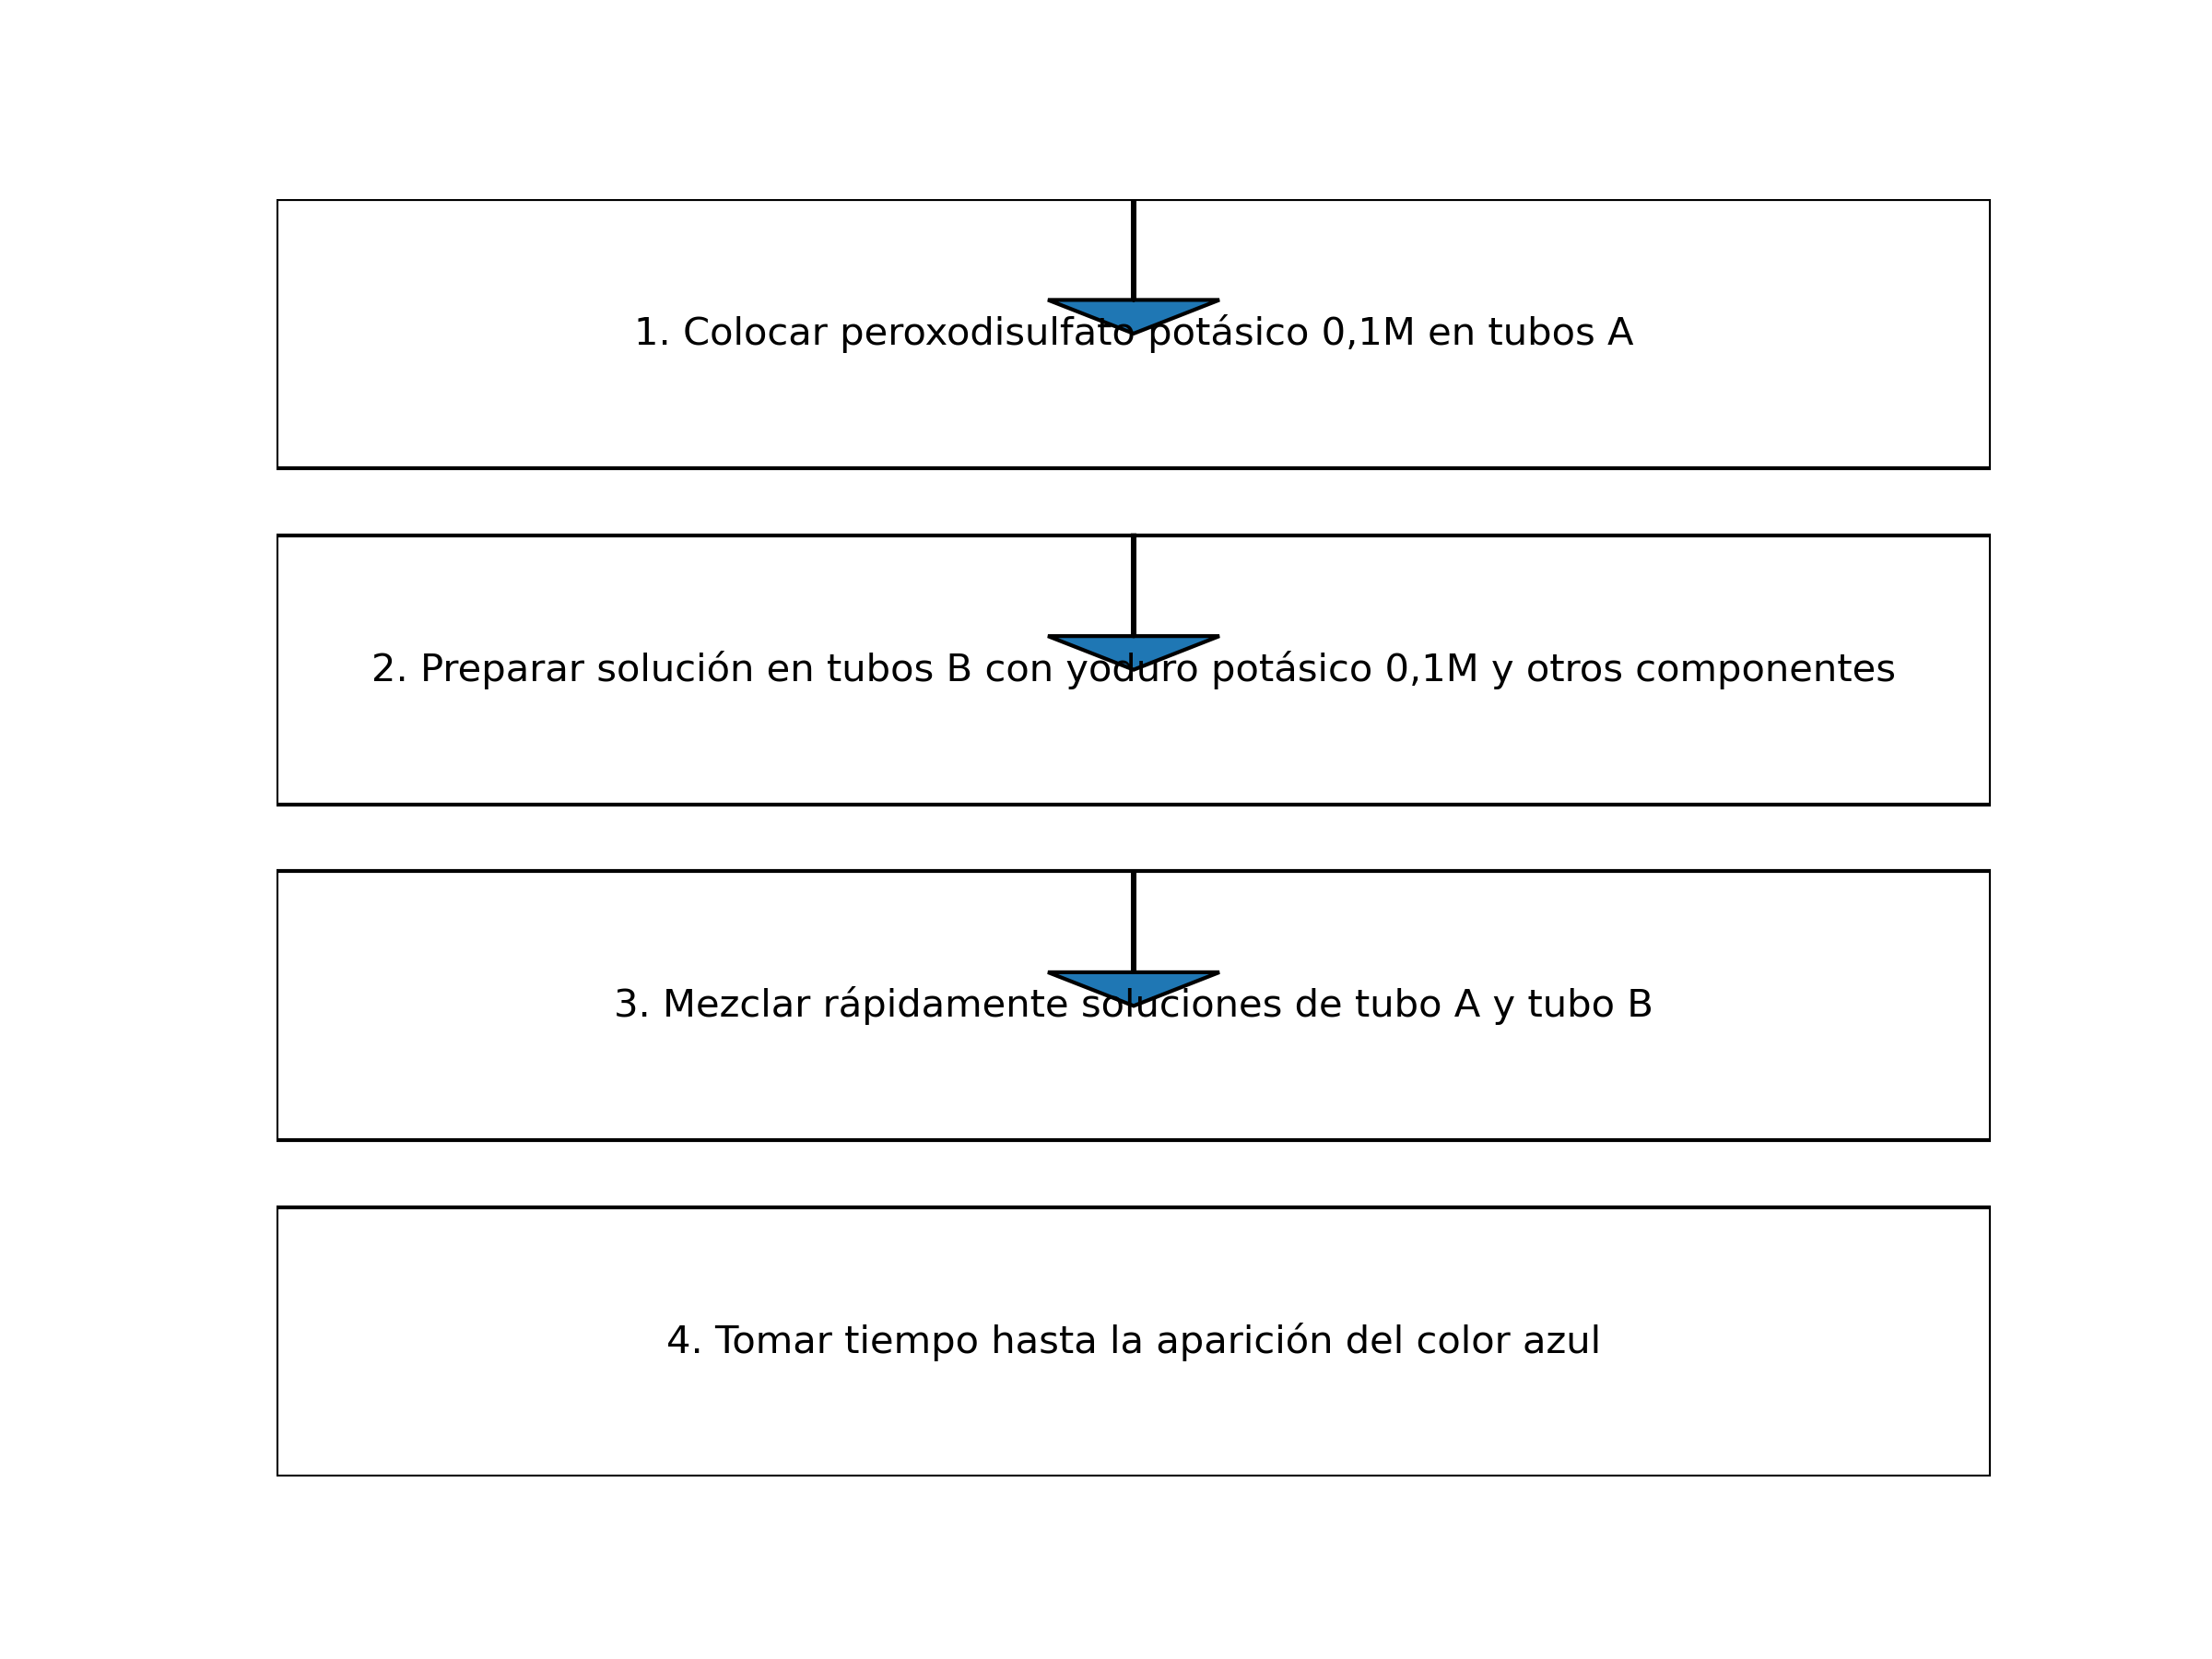
\includegraphics[width=0.8\textwidth]{diagrama_flujo.png}
\end{center}
\end{figure}

\section{Escriba todas las reacciones químicas balanceadas e indicando los estados de agregación, que se da en el experimento 1.}


\begin{equation}
\text{Tubo A: } \ce{K2S2O8(aq) -> 2K+(aq) + S2O8^2-(aq)}
\end{equation}

\begin{equation}
\text{Tubo B: } \ce{2KI(aq) + Na2S2O3(aq) + H2O(l) -> 2K+(aq) + 2Na+(aq) + I2(aq) + Na2S4O6(aq) + H2O(l)}
\end{equation}



\section{Cu\'al es la funci\'on que cumplen el almid\'on y el tiosulfato de sodio ($Na_{2} S_{2} O_{3}$), en el experimento 1?}
En el experimento 1, tanto el almidón como el tiosulfato de sodio (Na2S2O3) desempeñan roles importantes:

El almidón tiene la función de actuar como un indicador visual en el experimento. Cuando se combina con el yoduro potásico y el tiosulfato de sodio en el tubo B, el almidón sufre una reacción de descomposición debido a la liberación de yodo. Esta reacción produce un complejo de color azul oscuro con el yodo liberado, lo que nos permite detectar visualmente el momento en que la reacción ha finalizado. Observar el cambio de color a azul nos indica que el yodo ha sido liberado y, por lo tanto, que la reacción ha concluido.\cite{chang2005quimica}

Por otro lado, el tiosulfato de sodio (Na2S2O3) tiene la función de actuar como un agente reductor en el experimento. Al agregarlo al tubo B junto con el yoduro potásico, el almidón y el agua, el tiosulfato de sodio reacciona con el yodo liberado durante la reacción de oxidación del yoduro por el peroxodisulfato. Esta reacción evita que el yodo vuelva a reaccionar con el yoduro, lo cual permitiría obtener una determinación más precisa del tiempo necesario para que la reacción de oxidación se complete por completo.

En resumen, el almidón se utiliza como un indicador visual para detectar el final de la reacción mediante un cambio de color, mientras que el tiosulfato de sodio se emplea como un agente reductor para evitar reacciones secundarias entre el yodo liberado y el yoduro durante el experimento.

\begin{thebibliography}{99}

\bibitem{chang2005quimica}
Chang, Raymond.
\textit{Química}.
McGraw-Hill, 2005.




\end{thebibliography}




\end{document}
